%% start of file `cv_de.tex'.

% Preamble =================================================================================================
\documentclass[11pt, a4paper, roman]{moderncv}        % possible options include font size ('10pt', '11pt' and '12pt'), paper size ('a4paper', 'letterpaper', 'a5paper', 'legalpaper', 'executivepaper' and 'landscape') and font family ('sans' and 'roman')

% moderncv themes  -------------------------------------------------------------------------------------
\moderncvstyle[right]{casual} % style options are 'casual' (default), 'classic', 'banking', 'oldstyle' and 'fancy'
\moderncvcolor{blue}  % color options 'black', 'blue' (default), 'burgundy', 'green', 'grey', 'orange', 'purple' and 'red'
%\renewcommand{\familydefault}{\sfdefault}         % to set the default font; use '\sfdefault' for the default sans serif font, '\rmdefault' for the default roman one, or any tex font name
%\nopagenumbers{}                                  % uncomment to suppress automatic page numbering for CVs longer than one page

% character encoding
%\usepackage[utf8]{inputenc}                       % if you are not using xelatex ou lualatex, replace by the encoding you are using

% custom font --------------------------------------------------------------------------------------------
\usepackage{CormorantGaramond}

%\usepackage[T1]{fontenc}
%\usepackage{ebgaramond}

% additional packages  ------------------------------------------------------------------------------------
\usepackage{fontawesome5}
\usepackage[ngerman]{babel}
% \usepackage[absolute,overlay]{textpos} % for manual positioning of the photo
%\usepackage{lastpage}

% add page numbers
%\rfoot{\addressfont\itshape\textcolor{gray}{\thepage}}

% no hyphenation?
%\hyphenchar\font=-1
%\sloppy

% adjust the page margins  ------------------------------------------------------------------------------
\setlength{\footskip}{38pt}
\usepackage[left = 25mm, right = 20mm, top = 20mm, bottom = 25mm]{geometry}
\setlength{\hintscolumnwidth}{81pt}      % if you want to change the width of the column with the dates
%\setlength{\makecvheadnamewidth}{10cm}   % for the 'classic' style, if you want to force the width allocated to your name and avoid line breaks. be careful though, the length is normally calculated to avoid any overlap with your personal info; use this at your own typographical risks...

% define custom colors  ------------------------------------------------------------------------------
\definecolor{color0}{rgb}{0,0,0}% main default color, normally left to black
\definecolor{color1}{rgb}{0.22,0.45,0.70} % primary scheme color -> blue
\definecolor{color2}{rgb}{0,0,0} % secondary scheme color -> black
\definecolor{color3}{rgb}{0,0,0} % tertiary scheme color -> black

% renew commands if necessary -------------------------------------------------------------------------

% \cventry: omitted . at the end and italic font for second entry
\renewcommand*{\cventry}[7][.5em]{%
  \cvitem[#1]{#2}{%
    {\bfseries#3}%
    \ifthenelse{\equal{#4}{}}{}{, {#4}}%
    \ifthenelse{\equal{#5}{}}{}{, #5}%
    \ifthenelse{\equal{#6}{}}{}{, #6}%
    \strut%
    \ifx&#7&%
    \else{\newline{}\begin{minipage}[t]{\linewidth}\small#7\end{minipage}}\fi}}

% simple dash as first listitemsymbol
\renewcommand*{\listitemsymbol}{$-$ }

% spacing of cvlistitem
\renewcommand*{\cvlistitem}[2][.1em]{%
  \cvitem[#1]{}{\listitemsymbol\begin{minipage}[t]{\listitemcolumnwidth}#2\end{minipage}}}

% remove italic from recipient font
\renewcommand*{\addressfont}{\small\mdseries}
%
% % place photo below line
% \makeatletter
% \renewcommand*{\makecvhead}{% TODO: use \@initializecommand, which requires modifying its definition to handle \par
%   % recompute lengths (in case we are switching from letter to resume, or vice versa)
%   \recomputecvlengths%
%   % optional picture (pre-rendering)
%   \@initializebox{\makecvheadpicturebox}%
%   \savebox{\makecvheadpicturebox}{%
%     \ifthenelse{\isundefined{\@photo}}%
%       {}%
%       {\setlength\fboxrule{\@photoframewidth}%
%        \ifdim\@photoframewidth=0pt%
%          \setlength{\fboxsep}{0pt}\fi%
%        {\color{color1}\framebox{\includegraphics[width=\@photowidth]{\@photo}}}}}%
%   % name (pre-rendering)
%   \@initializelength{\makecvheadpicturewidth}%
%   \settowidth{\makecvheadpicturewidth}{\usebox{\makecvheadpicturebox}}%
%   \@initializebox{\makecvheadnamebox}%
%   \savebox{\makecvheadnamebox}{%
%     \parbox[b]{\textwidth-\makecvheadpicturewidth}{%
%       \if@left\raggedright\fi%
%       \if@right\raggedleft\fi%
%       \namefont%
%       \if@alternate% alternate design: first- and lastname in lowercase with no space in between (distinction is made by color difference)
%         {\color{color2!50}\MakeLowercase\@firstname}{\color{color2}\MakeLowercase\@lastname}%
%       \else% default design: first- and lastname as given with a space in between
%         {\color{color2}\@firstname} {\color{color2}\@lastname}\fi}}%
%   % rendering
%   \if@left%
%     \usebox{\makecvheadnamebox}
%           % optional title
%     \ifthenelse{\equal{\@title}{}}{}{%
%     %\\[.1em]\null% \null is required as there is no box on the line after \\, so glue such as \hfill (and leaders) disappear; this is in contrast to after \par, where the next line starts with an indent box (even after \noindent)
%     \if@right\hfill\fi%
%     \if@alternate%
%       \titlestyle{\MakeLowercase\@title}%
%     \else%
%       \hfill\titlestyle{\@title}\fi}\\[-.35em]%
%     {\color{color2!50}\rule{\textwidth}{.25ex}\vspace*{.5em}}
%     \null\hfill\usebox{\makecvheadpicturebox}\fi
%   \if@right%
%     \usebox{\makecvheadpicturebox}%
%     \usebox{\makecvheadnamebox}\fi\\[-.35em]%
%   %{\color{color2!50}\rule{\textwidth}{.25ex}}%
%   % optional detailed information
%   \if@details{%
%     \\\null%
%     \addressfont\color{color2}%
%     \ifthenelse{\isundefined{\@addressstreet}}{}{\addtomakeheaddetails{\addresssymbol\@addressstreet}%
%       \ifthenelse{\equal{\@addresscity}{}}{}{\addtomakeheaddetails[~--~]{\@addresscity}}% if \addresstreet is defined, \addresscity and \addresscountry will always be defined but could be empty
%       \ifthenelse{\equal{\@addresscountry}{}}{}{\addtomakeheaddetails[~--~]{\@addresscountry}}%
%         \flushmakeheaddetails\@firstmakeheaddetailselementtrue\\\null}%
%     \ifthenelse{\isundefined{\@born}}{}{\addtomakeheaddetails{\bornsymbol\@born}}%
%     \collectionloop{phones}{% the key holds the phone type (=symbol command prefix), the item holds the number
%       \addtomakeheaddetails{\csname\collectionloopkey phonesymbol\endcsname\collectionloopitem}}%
%     \ifthenelse{\isundefined{\@email}}{}{\addtomakeheaddetails{\emailsymbol\emaillink{\@email}}}%
%     \ifthenelse{\isundefined{\@homepage}}{}{\addtomakeheaddetails{\homepagesymbol\httpslink{\@homepage}}}%
%     \collectionloop{socials}{% the key holds the social type (=symbol command prefix), the item holds the link
%       \addtomakeheaddetails{\csname\collectionloopkey socialsymbol\endcsname\collectionloopitem}}%
%     \ifthenelse{\isundefined{\@extrainfo}}{}{\addtomakeheaddetails{\@extrainfo}}%
%     \flushmakeheaddetails}\fi% need to force a \par after this to avoid weird spacing bug at the first section if no blank line is left after \makehead
%   % optional quote
%   \ifthenelse{\isundefined{\@quote}}%
%     {}%
%     {{\null\hfill%
%       \begin{minipage}{\quotewidth}%
%         \centering%
%         \quotestyle{\@quote}%
%       \end{minipage}\hfill\null\\[2.5em]}}%
%   \par}
% \makeatother

% personal data ------------------------------------------------------------------------------------------
\name{}{Cornelius Hennch}
\title{Lebenslauf}                               % optional, remove / comment the line if not wanted
% \born{10.07.1992}                                 % optional, remove / comment the line if not wanted
% optional, remove / comment the line if not wanted; the "postcode city" and "country" arguments can be omitted or provided empty
% \address{}{}{}
% \phone[fixed]{}                  % optional, remove / comment the line if not wanted; the optional "type" of the phone can be "mobile" (default), "fixed" or "fax"
%\phone[fixed]{+2~(345)~678~901}
%\phone[fax]{+3~(456)~789~012}
\email{ cornelius.hennch[at]charite.de}
\homepage{ www.hennch.co}                       % optional, remove / comment the line if not wanted

% Social icons
% \social[linkedin]{john.doe}                        % optional, remove / comment the line if not wanted
% \social[twitter]{jdoe}                             % optional, remove / comment the line if not wanted
% \social[github]{corneliushennch}                   % optional, remove / comment the line if not wanted
% \social[orcid]{0000-0003-4104-5531}                  % optional, remove / comment the line if not wanted
% \social[researchgate]{Cornelius-Hennch}                        % optional, remove / comment the line if not wanted

% \extrainfo{additional information}                 % optional, remove / comment the line if not wanted

% photo --------------------------------------------------------------------------------------------------
\photo[80pt][0pt]{avatar.jpg}                       % optional, remove / comment the line if not wanted; '64pt' is the height the picture must be resized to, 0.4pt is the thickness of the frame around it (put it to 0pt for no frame) and 'picture' is the name of the picture file
%\quote{Some quote}                                 % optional, remove / comment the line if not wanted

% bibliography adjustments (only useful if you make citations in your resume, or print a list of publications using BibTeX)
%   to show numerical labels in the bibliography (default is to show no labels)
%\makeatletter\renewcommand*{\bibliographyitemlabel}{\@biblabel{\arabic{enumiv}}}\makeatother
\renewcommand*{\bibliographyitemlabel}{[\arabic{enumiv}]}
%   to redefine the bibliography heading string ("Publications")
%\renewcommand{\refname}{Articles}

% bibliography with mutiple entries
%\usepackage{multibib}
%\newcites{book,misc}{{Books},{Others}}

% Preamble end ==========================================================================================

%----------------------------------------------------------------------------------
%            content
%----------------------------------------------------------------------------------

\begin{document}

%-----       resume       ---------------------------------------------------------
\makecvtitle

% move text up
\vspace*{-20mm}
% manually placed photo ----> not very elegant
%  in cm:           (length from right, length from above)
%\begin{textblock}{0}(10.5,2) % <=======================================
%  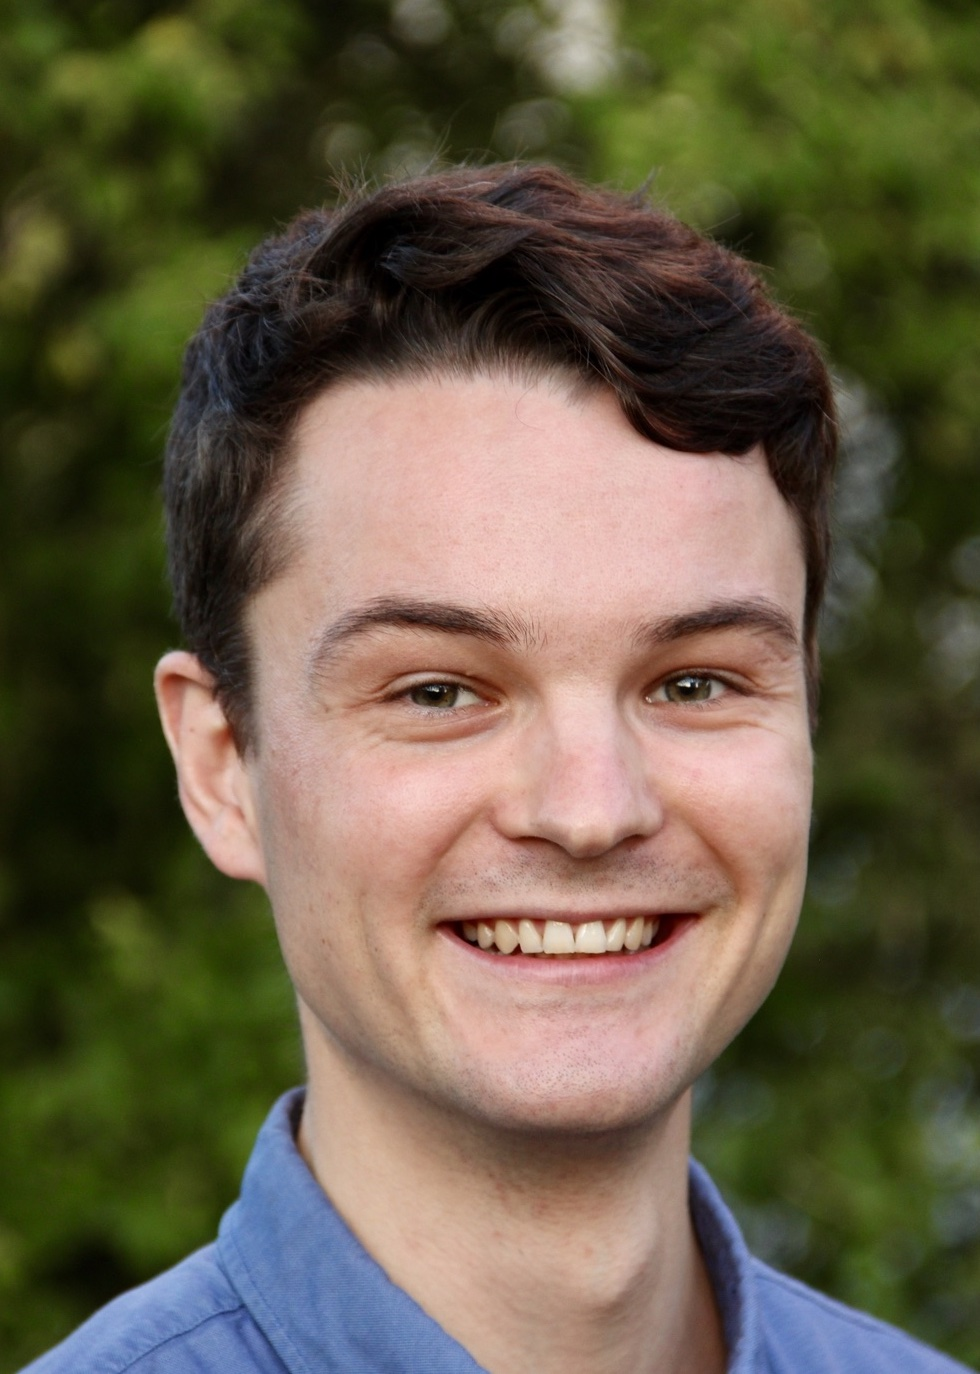
\includegraphics[width=90pt]{avatar.jpg}\par
%\end{textblock}

\section{Ausbildung / Akademischer Werdegang}
    \cventry{04/2013 -- 11/2020}{Studium der Humanmedizin}{Charité -- Universitätsmedizin Berlin}{}{}{Staatsexamen: Gesamtnote 1,0}
    %\cventry{07/2014 -- 11/2020}{Stipendium}{Studienstiftung des deutschen Volkes}{}{}{}
    \cvitem{07/2014 -- 11/2020}{\textbf{Stipendium} der Studienstiftung des deutschen Volkes}
    \cventry{10/2016 -- 06/2017}{Auslandsstudium (Erasmus)}{Université Paris Descartes (Paris V)}{Frankreich}{}{}
    \cventry{09/2002 -- 06/2011}{Abitur (Note 1,2)}{Robert-Bunsen-Gymnasium}{Heidelberg}{}{}

\subsection{Promotion}
\cventry{seit 09/2017}{Strukturiertes Promotionsstudium}{Berlin School of Integrative Oncology (BSIO)}{}{}{MD (Dr.med.) track}
\cvitem{Titel}{Identifikation und funktionelle Validierung neuer genetischer Mutationen im primär mediastinalen B-Zell Lymphom (PMBCL)}
\cvitem{Betreuer}{Prof. Dr. Frederik Damm, Dr. med. Daniel Nörenberg}
\cvitem{Abteilung}{Medizinische Klinik m. S. Hämatologie, Onkologie und Tumorimmunologie, Campus\newline{} Virchow Klinikum der Charité -- Universitätsmedizin Berlin}

% \newpage

\section{Klinische Praktika}

\subsection{Praktisches Jahr}
\cventry{06/2020 -- 10/2020}{PJ-Tertial Innere Medizin}{Campus Virchow Klinikum der Charité}{}{}{Medizinische Klinik m. S. Hämatologie, Onkologie und Tumorimmunologie, Station 51B und 51C, Schwerpunkt Leukämien und Lymphomerkrankungen}
\cventry{03/2020 -- 06/2020}{PJ-Tertial Chirurgie}{Vivantes Klinikum am Friedrichshain}{Berlin}{}{Klinik für Allgemein- und Viszeralchirurgie}
\cventry{11/2019 -- 03/2020}{PJ-Tertial Psychiatrie}{Zentrum für Psychiatrie Emmendingen (Lehrkrankenhaus der Albert-Ludwigs-Universität Freiburg)}{}{}{Klinik für Psychiatrie und Psychotherapie, Schwerpunkt psychotische Störungen}

% \newpage

\subsection{Famulaturen}
\cventry{09/2018}{Medizinische Klinik m. S. Hämatologie, Onkologie und Tumorimmunologie}{Campus Virchow Klinikum der Charité -- Universitätsmedizin Berlin}{}{}{Station 51B (Lymphomerkrankungen)}
\cventry{07/2017}{Allgemeinmedizinische Praxis}{Dr. Olaf Meyer}{Wedding, Berlin}{}{}
\cventry{10/2016 -- 06/2017}{Klinische Praktika während des Auslandsjahres}{Université Paris Descartes}{}{}{
\begin{itemize}
  \item[$-$] \textbf{Hôpital Cochin:} Interdisziplinäre Notaufname
  \item[$-$] \textbf{Hôpital St. Anne:} Psychiatrie und Neurologie
  \item[$-$] \textbf{Hôpital Necker:} Hämatologie, Gynäkologie/Geburtshilfe, Infektiologie und Pädiatrie
\end{itemize}}

\newpage

\cventry{04/2016}{Department of Anaesthesiology}{Queen Mary Hospital, Lehrkrankenhaus der University of Hong Kong}{Hong Kong S.A.R.}{}{}
\cventry{03/2016}{Department of Clinical Oncology}{Prince of Wales Hospital, Lehrkrankenhaus der Chinese University of Hong Kong}{Hong Kong S.A.R.}{}{}
\cventry{03/2015}{Klinik für Kardiologie, Angiologie und Pneumologie}{Universitätsklinikum Heidelberg}{}{}{Chest-Pain-Unit und kardiologische Ambulanz}

\section{Wissenschaftliche Praktika}
\cventry{09/2015 -- 01/2016}{Wissenschaftliche Arbeit (Modul 23)}{Labor für Strahlenbiologie, Klinik für Radioonkologie und Strahlentherapie, Charité}{Betreuung: Prof. Dr. Tinhofer-Keilholz}{}{Titel:  \emph{Molekulare und funktionelle Charakterisierung von Resistenzmechanismen im Zelllinienmodell des Kopf-Hals-Karzinoms}}


\section{Arbeitserfahrung}
\cventry{11/2014 -- 03/2021}{Studentischer Tutor}{Lernzentrum der Charité -- Universitätsmedizin Berlin}{}{}{Tutor für Problem-orientiertes Lernen (AG InterPOL)}
\cventry{08/2011 -- 08/2012}{Internationaler Jugendfreiwilligendienst (IJFD)}{Deutsch-Schweizerische Internationale Schule}{Hong Kong S.A.R.}{China}{}

% \section{Preise und Auszeichnungen}
% \cvitem{08/2010}{"`Outstanding achievement for international participants"' des „China Adolescents Science Technology and Inventions Contest 2010“ in Guangzhou, China}
% \cvitem{05/2010}{Sonderpreis des Bundeswettbewerbs „Jugend forscht“ in der Kategorie Biologie}


\section{Außercurriculäre Aktivitäten}
\subsection{Engagement}
\cvitem{seit 10/2020}{Engagement bei Health for Future Berlin, Leitung des Reflektionstreffens der Planetary\newline{}Health Academy 2020/21}
\cvitem{06/2018 -- 10/2019}{Mitarbeit in der AG „Neue Impulse für die Forschung an der Charité“ am QUEST Center des Berlin Institute of Health (BIH)}
\cvitem{10/2017 -- 11/2020}{Studentischer Vertreter in Berufungs- und Habilitationskommissionen}
\cvitem{10/2015 -- 07/2016}{Gründung und Leitung eines interdisziplinären studentischen Journal Clubs an der Charité}
\cvitem{02/2014 -- 07/2016}{Studentischer Vertreter in der Nachwuchs- und Forschungskommission der Charité}
\cvitem{02/2014 -- 03/2015}{Referent für Öffentlichkeitsarbeit und Sitzungsleitung der FSI Medizin der Charité}
\subsection{Kongresse}
\cvitem{03/2021}{6th DKTK Berlin Cancer Retreat (Abstract talk)}
\cvitem{07/2018}{Cambridge Lymphoma Biology International Symposium (Teilnahme)}
\subsection{Kurse und Seminare}
\cvitem{seit 09/2017}{Regelmäßige Teilnahme an Veranstaltungen des "`Berlin Epidemiological Methods\newline{}Colloquium"' (BEMC)}
\cvitem{05/2018 - 06/2019}{"`Reproducible Research with R"' Kurse des QUEST Center (Basic, Advanced und Applied)}
\cvitem{08/2018}{Sommerakademie der Studienstiftung, Kursthema: "`The third wave of behavioral therapy"'}

% \cvitem{12/2017 -- 02/2018}{Statistikkurs "`Navigating Numbers"'}
% \cvitem{02/2021 -- 04/2021}{Nature Masterclass „Scientific Writing"}
% \newpage

\section{Sprachkenntnisse}
\cvitemwithcomment{Französisch}{Niveau C2}{}
\cvitemwithcomment{Englisch}{Niveau C2}{IELTS score 8,5/9}
% \cvitemwithcomment{Kantonesisch}{Erweiterte Grundkenntnisse}{}

\newpage

%\section{Computer skills}
%\cvdoubleitem{category 1}{XXX, YYY, ZZZ}{category 4}{XXX, YYY, ZZZ}
%\cvdoubleitem{category 2}{XXX, YYY, ZZZ}{category 5}{XXX, YYY, ZZZ}
%\cvdoubleitem{category 3}{XXX, YYY, ZZZ}{category 6}{XXX, YYY, ZZZ}

\section{Fähigkeiten}
\cvitem[.1em]{Datenanalyse}{\textbf{Statistisches Programmieren mit R}} %\faRProject
  \cvlistitem{Bereinigung und Transformation von klinischen/molekularen Datensätzen}
  \cvlistitem{Vielfältige Visualisierungen (z.B. mit \texttt{ggplot2})}
  \cvlistitem[.25em]{Reproduzierbare Analysen mit RMarkdown/Github}
\cvitem[.1em]{}{\textbf{Statistische Methoden}}
  \cvlistitem{Deskriptive Statistik}
  \cvlistitem[.25em]{Analyse klinischer Daten mit Regressionsmodellen}
\cvitem[.1em]{Experimentelle Methoden}{\textbf{Zelllinienmodelle}\newline{} -- Genome editing (Knock-out und Knock-in) mit CRISPR/Cas9\newline{} -- funktionelle Assays}%{\cvskill{3}}
%  \cvlistitem{Genome editing (Knock-out und Knock-in) mit CRISPR/Cas9}
%  \cvlistitem[.25em]{funktionelle Assays}
\cvitem{}{\textbf{Next-Generation sequencing (NGS)}}%{\cvskill{2}}
  \cvlistitem{AmpliconSeq}
  \cvlistitem{Targeted re-sequencing}
%{\cvskill{2}}

%\section{References}
%\begin{cvcolumns}
%  \cvcolumn{Category 1}{\begin{itemize}\item Person 1\item Person 2\item Person 3\end{itemize}}
%  \cvcolumn{Category 2}{Amongst others:\begin{itemize}\item Person 1, and\item Person 2\end{itemize}(more upon request)}
%  \cvcolumn[0.5]{All the rest \& some more}{\textit{That} person, and \textbf{those} also (all available upon request).}
%\end{cvcolumns}

% Publications from a BibTeX file without multibib
%  for numerical labels: \renewcommand{\bibliographyitemlabel}{\@biblabel{\arabic{enumiv}}}% CONSIDER MERGING WITH PREAMBLE PART
%  to redefine the heading string ("Publications"):
\renewcommand{\refname}{Publikationen}
\nocite{*}
\bibliographystyle{abbrv}
\bibliography{my_publications}

\section{Interessen und Hobbies}
\cvitem{}{Rennrad fahren, Segeln, Lesen, klassische Konzerte und Theater}\bigskip

% Publications from a BibTeX file using the multibib package
%\section{Publications}
%\nocitebook{book1,book2}
%\bibliographystylebook{plain}
%\bibliographybook{publications}                   % 'publications' is the name of a BibTeX file
%\nocitemisc{misc1,misc2,misc3}
%\bibliographystylemisc{plain}
%\bibliographymisc{publications}                   % 'publications' is the name of a BibTeX file

Berlin, \today\\[.5em]
% \includegraphics[width=6cm]{Unterschrift.pdf}\\[.5em]
Cornelius Hennch

\end{document}


%% end of file `template.tex'.

